% Evie Lives here
\section{systemd Services}
systemd is a service manager, which is a program that launches and monitors different services across the system. The digital-ink application is automatiacally started upon boot by the systemd process, which ensures that the application is started correctly and without errors. If any errors occur, systemd will log them in a tool known as journalctl and then follow a configuration file for instructions on how to handle those errors. This can range from simply restarting a program that has errored, to trying once again, or recording the failure and performing no action.

\begin{figure}
    \centering
    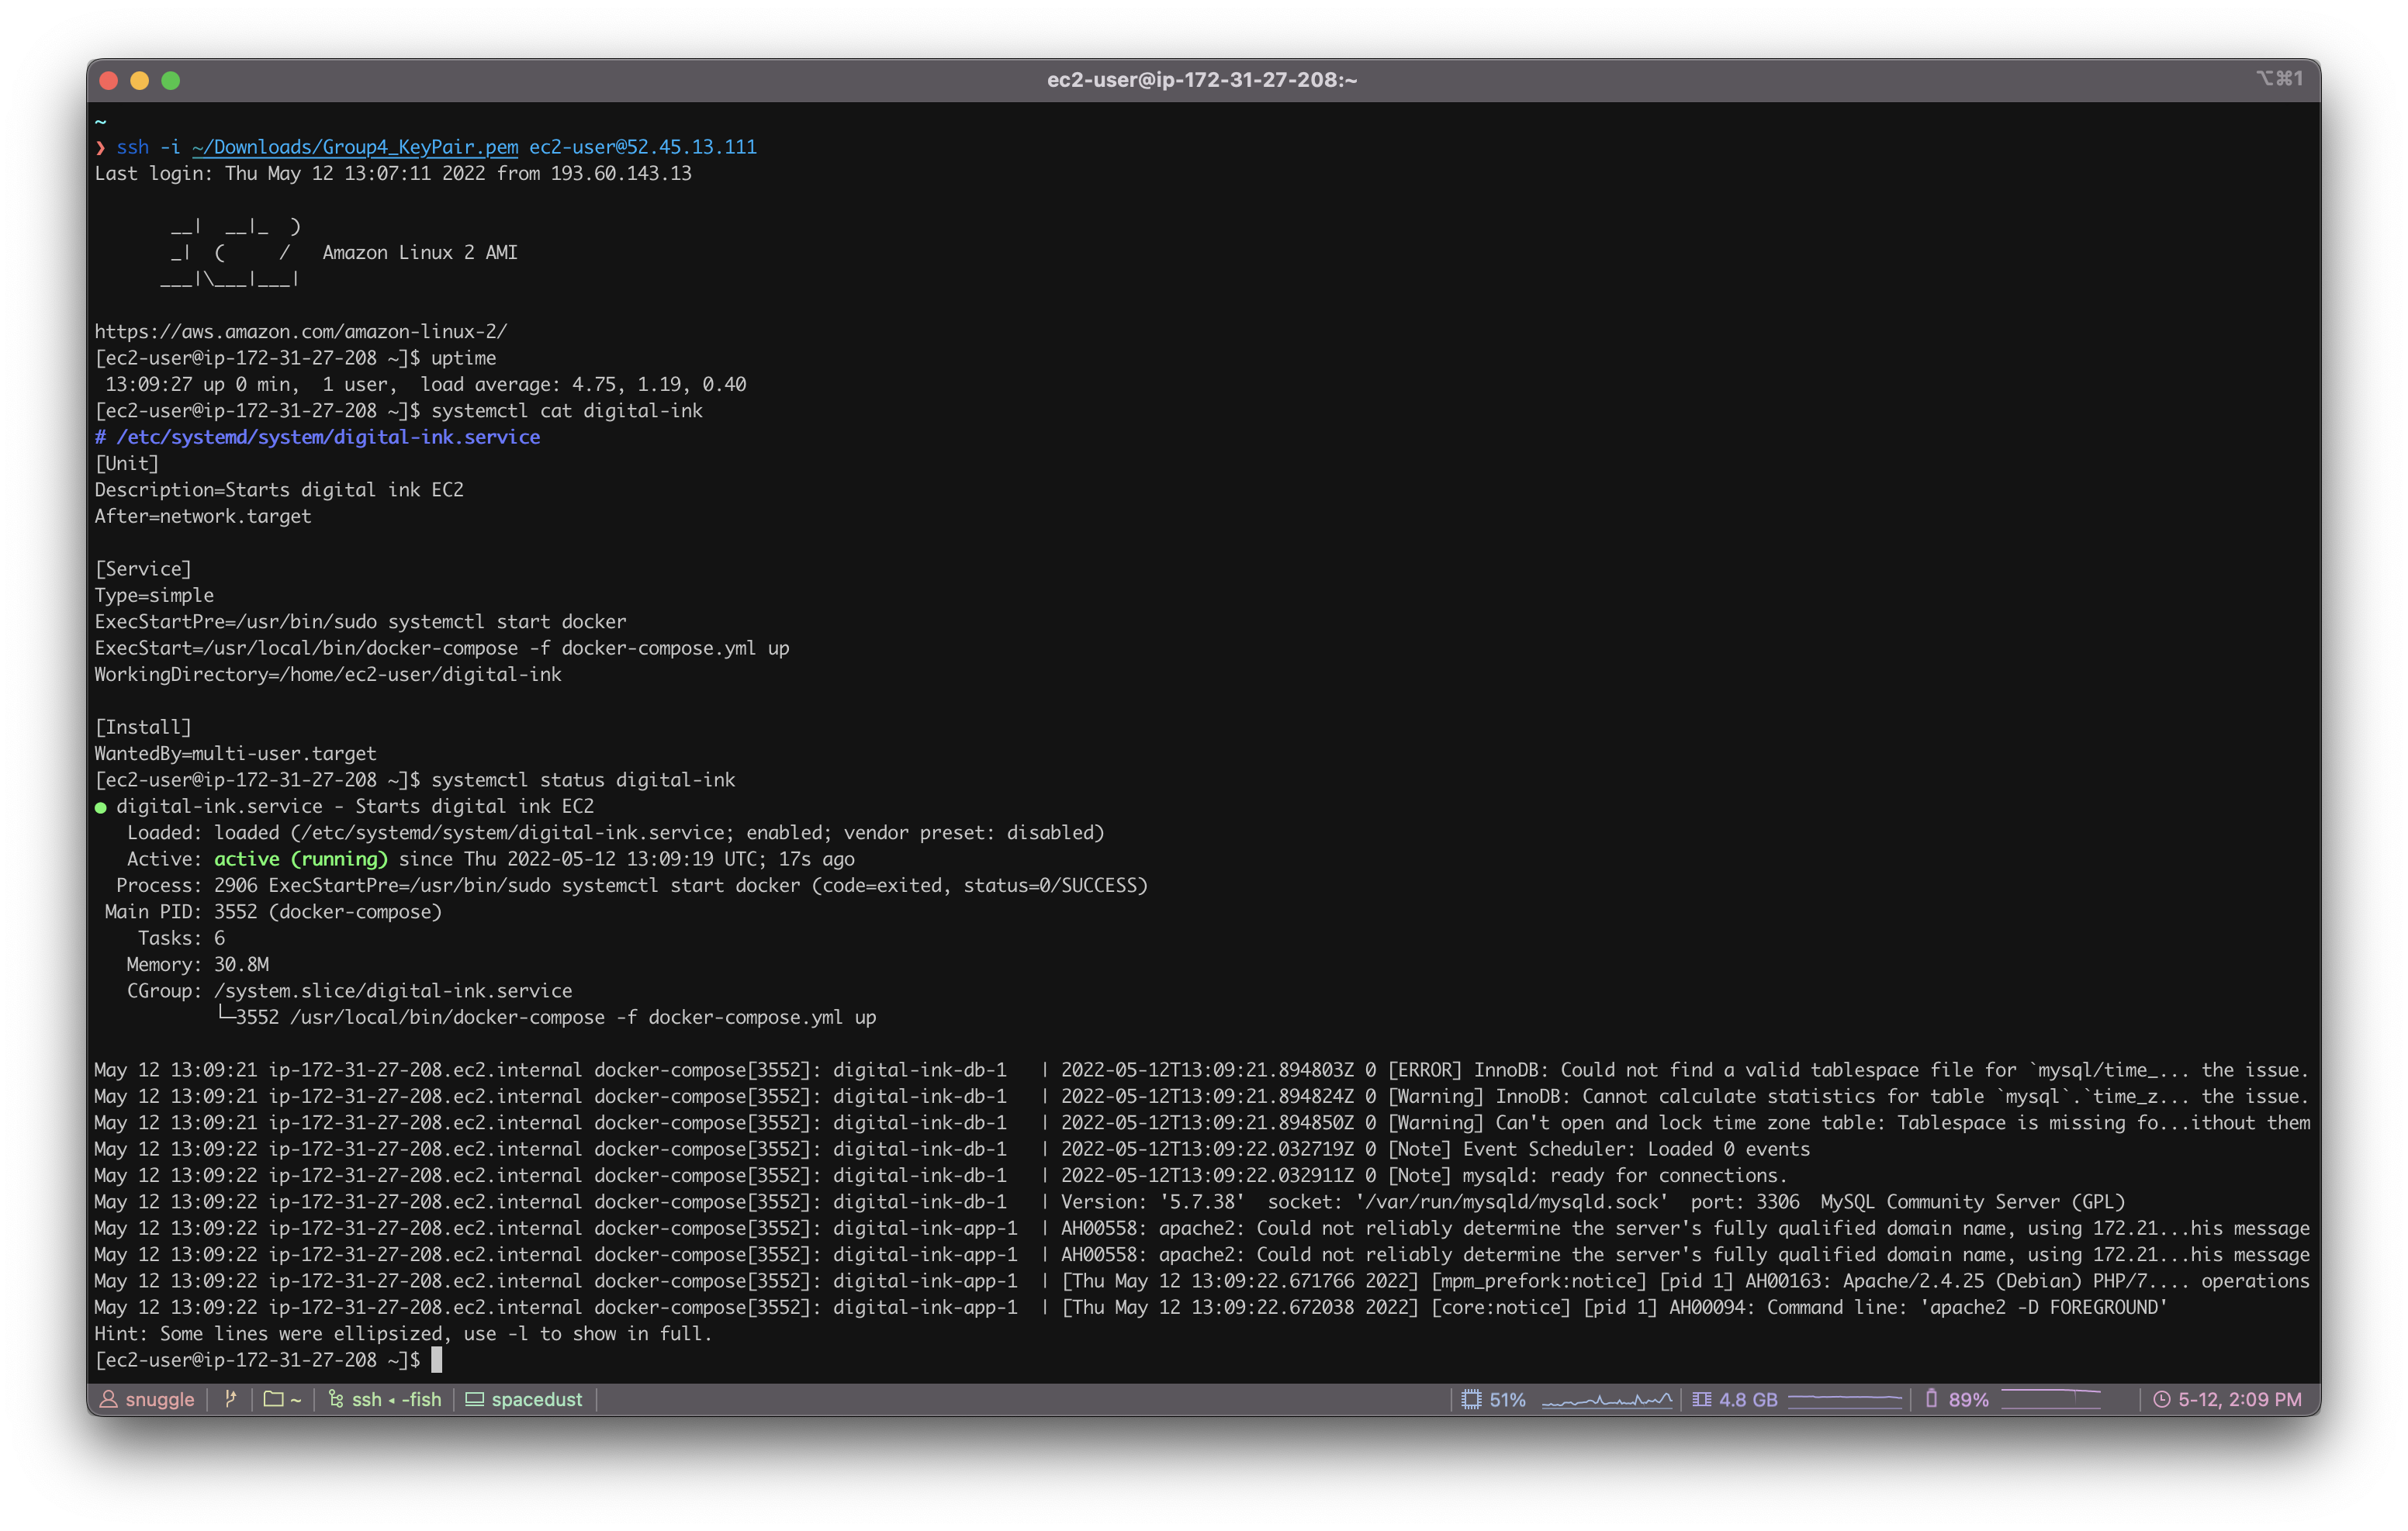
\includegraphics[width=\textwidth]{resources/systemd/systemd.png}
    \caption{Creation of systemd Service}
    \label{fig:systemd}
\end{figure}
